\documentclass[11pt]{article}

% Generic, dependency-light preprint/workshop-short-paper format.
% No venue-specific .cls required -- compiles as-is on Overleaf or any
% standard TeX Live install (texlive-latex-base + texlive-latex-extra).
% Swap in an official venue template later; content/citations are the
% part that took the work, not the final formatting.

\usepackage[margin=1in]{geometry}
\usepackage{graphicx}
\usepackage{booktabs}
\usepackage{amsmath}
\usepackage{amssymb}
\usepackage[hidelinks]{hyperref}
\usepackage{xcolor}
\usepackage{enumitem}

\newcommand{\todo}[1]{\textcolor{red}{[TODO: #1]}}

\title{The Occupancy Curve: A Support-Stratified Evaluation of LLM Note Placement}
\author{\todo{author names} \\ \todo{affiliation}}
\date{Draft --- \today. Not anonymized. 4-page short-paper target.}

\begin{document}
\maketitle

\begin{abstract}
When an LLM agent files a new note into an existing folder hierarchy,
prior work does not report accuracy as a function of how many notes
already sit in the target folder (its \emph{support}) --- nor does it
evaluate folders with no prior notes at all. We stratify by support
directly and find that method rankings differ by stratum: a frontier
model prompted with the full folder tree stays in a narrow band, a
retrieval baseline is consistently above it, and a fine-tuned small model
crosses both. We validate our gold labels with a two-annotator study
(Cohen's $\kappa=0.901$). On a second corpus we also stratify by support
directly, and on a third; in the item-stratified regime shared by all
three, a fine-tuned model beats the retrieval-then-pick cascade that wins
on our first corpus --- a reversal reproduced on both additional corpora,
whose cause we tested for (a proposed tree-size mechanism) and did not
find. We report the reversal as real and its cause as open, rather than
force an explanation onto it. Support strata are confounded with folder,
vault, and corpus identity --- we do not claim support causes the
ranking change, only that it correlates with it and the correlation
reproduces where we have the data to check.
\end{abstract}

\section{Introduction}

Write-time filing --- given a new note and an existing folder tree, which
folder should it join --- is a small, concrete instance of the broader
agent-memory-organization problem. It has a clean metric (does the
model's predicted path match where the note was actually filed) and a
natural axis the literature has not stratified results by: how much
evidence already exists for the target folder. A folder with fifteen
similar notes in it is evaluated identically to a folder with zero in
existing work, even though nothing guarantees a method that's good at one
is good at the other.

PaperRouter-Agent~\cite{paperrouter} names this task PHPR
and reports a cascade of retrieval and LLM inspection beating a flat
baseline by 22 points on five researchers' Zotero libraries. Their
pipeline already formalizes folders by their existing members and
abstains when membership is too thin, but does not report accuracy
\emph{as a function of} member count and does not evaluate folders with
zero members. We do not know, and do not claim to know, whether their
support distribution skews toward well-populated folders --- only that
they do not report the stratified breakdown, and we do.

We stratify by support directly. Figure~\ref{fig:fig1} shows the result
on our primary corpus: a frontier model given the full folder list
(\textbf{flat}) stays in a narrow band across the item-stratified support
strata; a \textbf{k-nearest-neighbor} retrieval baseline sits
consistently above it at every positive-support stratum; a
\textbf{fine-tuned 8B model} crosses both. The disconnected zero-support
point (a separately constructed evaluation, see \S\ref{sec:method}) is
not comparable to the item-stratified strata as a ``band width'' --- it
comes from a different split with different method configurations
entirely --- but it is itself informative: all three methods are much
closer to each other there than anywhere else on the item-stratified
side, a fourth regime prior work has not reported on at all, not just an
underreported tail of the one it does.

\paragraph{Contributions.}
\begin{enumerate}[leftmargin=*, itemsep=2pt]
  \item A support-stratified evaluation for note placement, including a
    zero-support (folder-disjoint) regime existing work does not
    evaluate.
  \item A candidate-set-size $\times$ grounding factorial
    (\S\ref{sec:grounding}) that is suggestive, not decisive, about which
    part of PaperRouter-Agent's reported gain a retrieval step alone
    could plausibly account for.
  \item Cross-corpus evidence (two independent public corpora, 43
    vaults/repos total, item-stratified split) that a fine-tuned model
    beats a retrieval-then-pick cascade in a regime where our own
    private corpus shows the opposite ranking --- a real, reproduced
    reversal whose cause we test for and do not find
    (\S\ref{sec:reversal}). One of the two public corpora also has a
    folder-disjoint result, and it does \emph{not} show this reversal
    (\S\ref{sec:reversal}, \S\ref{sec:discussion}) --- the reversal is
    specific to the seen-folder regime, on the evidence we have.
  \item A two-annotator gold-label validation study, $\kappa=0.901$, on
    whether our corpus-A gold labels are sensible destinations --- not a
    validation of the exact-match metric's single-correct-answer
    assumption, which the study does not test (\S\ref{sec:annotation}).
\end{enumerate}

\begin{figure}[t]
  \centering
  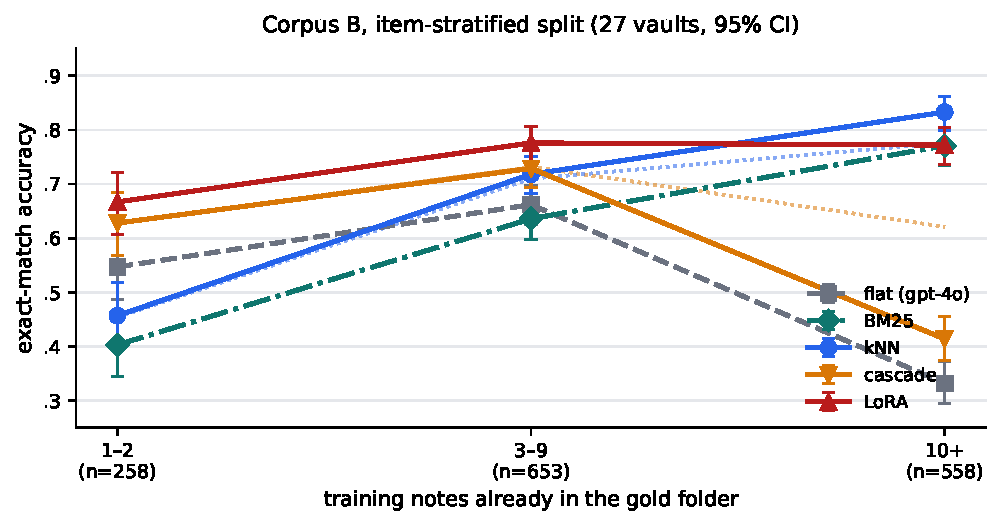
\includegraphics[width=0.92\linewidth]{figures/fig1_coverage_curve.pdf}
  \caption{Corpus A. The $x=0$ point comes from a separately constructed
  folder-disjoint split with different method configurations
  (\S\ref{sec:method}) and is plotted disconnected from the
  item-stratified strata ($x=1..3$) --- it is not the left edge of one
  fitted curve, and its spread should not be compared to theirs as if it
  were. 95\% Wilson-score confidence intervals shown per point (marginal
  per-point intervals, not a test of the between-point difference);
  $n=18$ at the 1--2 stratum is the point to read most cautiously. gpt-4o
  given the full folder list stays in a narrow band across the
  item-stratified strata; kNN sits above it at every one of those
  strata; LoRA crosses both flat and kNN. The kNN/LoRA 1--2-vs-3--9 gap
  is small relative to their wide, overlapping intervals at $n=18$ ---
  read as inconclusive at that stratum, not as evidence either way.}
  \label{fig:fig1}
\end{figure}

\section{Related Work}

\paragraph{PaperRouter-Agent~\cite{paperrouter}.} Same task (they call it
PHPR), flat 0.39 $\to$ agent 0.61 on five Zotero libraries. No
unseen-folder evaluation, no retrieval-only baseline, no fine-tuned
baseline, and no support-stratified breakdown --- our contribution is the
missing axis, not a new task.

\paragraph{Filesystem-as-Memory~\cite{filesystem-memory}.} Finds that
organizing agent memory as a folder tree does not itself improve
downstream answer accuracy; organization pays for itself in retrieval
cost, not correctness. We do not claim placement quality improves
answers --- our metric is purely ``did the file land where it actually
sat,'' not any downstream task.

\paragraph{MemDelta~\cite{memdelta}.} A one-variable-at-a-time protocol
paper showing a single unreported hidden variable can flip a
memory-system's reported conclusions. Its methodological caution is why
we run more than one model family (gpt-4o and Llama-3.3-70B) and report
every protocol axis (prompt token counts, candidate-set sizes, split
construction) rather than a single number.

\paragraph{Zero-shot extreme multi-label classification} (ZestXML,
SemSup-XC, and related work) routinely evaluates unseen-label splits. The
folder-disjoint split we use is not a novel method --- it is standard
practice one field over that this literature has not adopted.

\section{Task and Method}
\label{sec:method}

\paragraph{Task.} Given a note's text and a folder tree, predict the
folder path the note belongs in. We score exact path match against the
note's actual folder-of-record.

\paragraph{Support.} For a given train/val split, a val item's
\emph{support} is the number of training-partition notes already filed
in its gold folder. We bucket into $\{0, 1\text{--}2, 3\text{--}9,
10{+}\}$. \textbf{These buckets are not one continuous curve --- they
come from two separately constructed splits of the same underlying task
pool}, and the methods evaluated on each are configured differently,
described below. Zero support comes from a folder-disjoint split (entire
folders held out of training, guaranteeing zero support by construction,
verified on every corpus). Positive support comes from a separate
item-stratified split (folders seen in training, individual notes held
out). We report both in one table for space, but treat the zero-support
point as a distinct experiment, not the left edge of a fitted curve --- a
limitation we return to in \S\ref{sec:discussion}, and a reason
Figure~\ref{fig:fig1} does not connect it to the rest of the line.

\paragraph{Methods compared, item-stratified split (support $>0$).}
(1)~\textbf{Flat}: full folder list in the prompt, gpt-4o. (2)~\textbf{kNN}:
embed the new note, retrieve its nearest neighbors among training notes,
predict their folder (majority vote; $k=5$). Zero by construction on the
0-support bucket --- it can only predict folders that have a training
example. (3)~\textbf{Cascade}: embedding shortlist of the top-20 folders
by nearest-training-note similarity, then an LLM pick from the shortlist
--- same prompt/parser as flat, only the candidate list changes.
(4)~\textbf{LoRA}: llama-3.1-8b, LoRA rank 16, 1 epoch, fine-tuned on the
item-stratified train split, full folder list at inference (matches
flat's information, not cascade's).

\paragraph{Methods compared, folder-disjoint split (support $=0$),
corpus A only.} Because no training note exists in an unseen folder,
kNN's note-based shortlist is empty by construction and the cascade
instead uses a folder-\emph{path-string} embedding shortlist (top-50, not
top-20 --- chosen because it has substantially higher recall against
unseen folders on this corpus), and LoRA is a \textbf{separately
fine-tuned model} trained on the folder-disjoint split's own train
partition, not the same checkpoint used for the positive-support buckets.
The zero-support row in every table in this paper is therefore not ``the
same four methods extrapolated to zero'' --- it is a different cascade
configuration and a different LoRA checkpoint, evaluated on a genuinely
different task (generalizing to a folder with no exemplar at all).

\paragraph{Corpora.} Corpus A: one person's private working directory,
870 tasks across 170 folders that actually hold a task (the model is
offered the larger set of 365 candidate folders that exist in the tree,
most of them empty of training/val tasks), 78\% one software project
(\texttt{work/openclaw}) --- see \S\ref{sec:discussion} for the
construct-validity implication. Corpus B: 27 public personal markdown
note vaults (GitHub; 14/27 use Obsidian specifically, the rest are plain
markdown note collections), 4{,}199 tasks, mean 39 folders/vault,
selected and filtered by a two-stage classifier (structural thresholds
alone cannot separate personal note vaults from software repositories
that happen to ship markdown --- package-manifest and source-file-count
signals can; see Appendix~\ref{app:classifier}). Corpus B also has a
folder-disjoint evaluation, reported in \S\ref{sec:reversal} alongside
its item-stratified result --- item-stratified is still where this
paper's headline results live. Corpus A$'$: 16 public software
repositories, 2{,}644 tasks, mean 63 folders/repo. A$'$'s folder-disjoint
split data was built but never evaluated (no method was run on it) ---
an explicit scope choice, not a null result; A$'$ contributes
item-stratified results only in this paper. All corpora pin commit SHAs;
note text is never redistributed, aggregate statistics only.

\section{Results}

\subsection{Accuracy by support stratum (corpus A)}
\label{sec:coverage}

\begin{table}[h]
  \centering
  \small
  \begin{tabular}{lrrrr}
    \toprule
    support & $n$ & flat (gpt-4o) & kNN & LoRA \\
    \midrule
    0     & 353 & 0.354 & 0.000 & 0.363 \\
    1--2  & 18  & 0.278 & 0.444 & 0.222 \\
    3--9  & 105 & 0.200 & 0.381 & 0.371 \\
    10+   & 171 & 0.339 & 0.620 & 0.673 \\
    \bottomrule
  \end{tabular}
  \caption{Accuracy by support stratum, corpus A.}
  \label{tab:coverage}
\end{table}

Within the item-stratified split (1--2/3--9/10+), flat stays in a narrow
band (.20--.34); kNN sits above flat at every one of these three strata
(never crosses it); LoRA crosses both flat and kNN, below flat at 1--2
and above both flat and kNN by 10+. The 1--2 vs.\ 3--9 movement for kNN
and LoRA is not distinguishable from noise given their wide, overlapping
intervals at $n=18$ (Figure~\ref{fig:fig1}) --- read the exact ordering
within that pair as inconclusive. A fourth method, the retrieval-then-pick
cascade (embedding shortlist $\to$ gpt-4o), was not broken down by
support stratum, but wins on both splits taken as wholes: 0.643 vs.\
0.537 (LoRA) pooled across the item-stratified split ($n=294$,
$p=0.00045$, paired), and 0.419 vs.\ 0.363 on the separately constructed
zero-support split ($n=353$, $p=0.040$, paired) --- no training required
to beat the fine-tuned model on either. These $p$-values, and every
$p$-value in this paper computed on corpus A, come from a single tree
(corpus A has one folder hierarchy), so they describe this corpus's
items, not a population of trees; we do not treat them as evidence the
result generalizes --- \S\ref{sec:reversal} tests that directly and
finds it does not, in this ranking's specific direction.

\subsection{Candidate-set size $\times$ grounding factorial}
\label{sec:grounding}

A $2\times2$ factorial, corpus A, item split ($n=294$, paired, single
tree --- same single-tree caveat as \S\ref{sec:coverage}). The two
factors are candidate-set size (365 folders vs.\ a retrieved top-20) and
grounding (whether each candidate folder carries a one-line description).
We call it a factorial because both factors are crossed in the design
below, not because either factor is internally decomposed --- cutting the
candidate list to a retrieved top-20 is one bundled intervention (it
changes what's retrieved, the candidate count, and prompt length
together), not an isolation of retrieval as a mechanism.

\begin{table}[h]
  \centering
  \small
  \begin{tabular}{lcc}
    \toprule
    & no descriptions & + descriptions \\
    \midrule
    flat (365 folders)   & 0.286 & 0.306 ($p=0.489$, ns) \\
    retrieved top-20     & 0.643 & 0.660 ($p=0.487$, ns) \\
    \bottomrule
  \end{tabular}
  \caption{Candidate-set-size $\times$ grounding factorial.}
  \label{tab:factorial}
\end{table}

Moving from the flat row to the retrieved-top-20 row is associated with
+35pt in both columns; adding a one-line folder description within either
row is within noise --- failure to reject at $n=294$, not evidence the
two conditions are equivalent. This is suggestive about PaperRouter-Agent's
reported +22pt gain, not decisive: our grounding condition is a one-line
summary from at most four truncated notes, not their full top-down
planning and type-aware member inspection, and our candidate-set-size
factor is a bundled intervention as noted above --- we cannot separate a
pure retrieval effect from a pure list-shortening effect here, so we do
not claim to have identified which of their pipeline stages drives their
number.

\subsection{Cross-corpus generalization, item-stratified split only}
\label{sec:reversal}

The same cascade-vs-LoRA comparison on two independent public corpora,
\textbf{item-stratified split} (the regime \S\ref{sec:coverage} covers;
see below for what corpus B's folder-disjoint split shows):

\begin{table}[h]
  \centering
  \small
  \begin{tabular}{lccl}
    \toprule
    corpus & LoRA & cascade & vault-level win count \\
    \midrule
    A (private, 1 tree)     & 0.537 & \textbf{0.643} & n/a --- one tree \\
    B (27 personal vaults)  & \textbf{0.756} & 0.592 & LoRA 19/27, cascade 6, tie 2 \\
    A$'$ (16 software repos) & \textbf{0.716} & 0.552 & LoRA 13/16, cascade 3/16, tie 0 \\
    \bottomrule
  \end{tabular}
  \caption{Cross-corpus LoRA vs.\ cascade, item-stratified split.}
  \label{tab:crosscorpus}
\end{table}

Cascade wins on A; LoRA wins on both B and A$'$ on this split, and the
win is broad at the vault level on both --- not a pooled-average artifact
of a few vaults. Corpus B's own support-stratified breakdown (analogous
to Table~\ref{tab:coverage}, kNN at $k=5$, cascade path@20) replicates
the crossing pattern, not just the aggregate:

\begin{table}[h]
  \centering
  \small
  \begin{tabular}{lrrrrr}
    \toprule
    support & $n$ & flat (gpt-4o) & kNN & cascade & LoRA \\
    \midrule
    1--2  & 258 & 0.547 & 0.457 & 0.628 & 0.667 \\
    3--9  & 653 & 0.662 & 0.718 & 0.729 & 0.776 \\
    10+   & 558 & 0.332 & \textbf{0.833} & 0.414 & 0.772 \\
    \bottomrule
  \end{tabular}
  \caption{Accuracy by support stratum, corpus B (item-stratified).}
  \label{tab:corpusb}
\end{table}

LoRA leads at 1--2 and 3--9; kNN overtakes everything, including LoRA, at
10+ --- cascade never leads any stratum on corpus B, unlike on corpus A
where it wins pooled. This is genuine stratum-level replication of ``the
ranking is not what corpus A showed,'' not merely the same aggregate
number restated. \textbf{This does not hold on the folder-disjoint
split.} Corpus B's zero-support evaluation shows cascade beating LoRA
there too (0.583 vs.\ 0.475) --- the same ranking as corpus A, not the
reversal. (A$'$'s folder-disjoint split data exists but was never
evaluated with any method --- an explicit scope choice, not a null
result; see \S\ref{sec:discussion}.) The reversal reported here is
specific to the item-stratified, seen-folder regime and should not be
read as ``LoRA wins on public corpora'' without that qualifier. A$'$ has
no support-stratified breakdown of its own in this paper (item-split
aggregate only, by design, \S\ref{sec:method}) --- for A$'$ we can say
the aggregate item-split reversal replicates; only corpus B lets us also
say the stratum-level crossing pattern replicates.

We hypothesized tree size as the mechanism for the item-stratified
reversal (smaller trees favor a model that sees the whole folder list;
larger trees favor a shortlist-based cascade) and tested it directly: a
permutation test on the correlation between each vault's folder count and
its (LoRA $-$ cascade) margin, at the vault level --- the correct unit,
since items within a vault are not independent draws.

\begin{center}
\small
\begin{tabular}{lrrr}
\toprule
 & $n$ & Spearman(log-folders, margin) & $p$ \\
\midrule
corpus B  & 27 & $+0.029$ & 0.887 \\
corpus A$'$ & 16 & $-0.115$ & 0.669 \\
pooled    & 43 & $+0.034$ & 0.826 \\
\bottomrule
\end{tabular}
\end{center}

Null in both corpora, opposite-signed between them. \textbf{We found no
evidence that tree size explains the margin} --- a null result at
$n=27/16$, not proof the effect is zero. An earlier version of this
analysis, pooling items across vaults into three folder-count bins,
showed a strong, monotone, ``significant'' pattern ($p$ as low as
$10^{-25}$) --- an artifact of treating correlated items as independent
draws, caught before this pattern was reported as a finding. We report
the item-stratified reversal as real (broad, vault-level, reproduced on
two corpora) and its cause as genuinely open. Candidate explanations we
have not ruled out, and consider at least as likely as tree size: the two
public corpora pool training data across many vaults into one fine-tuned
model, so the win could reflect total training volume or cross-tree
transfer rather than anything about individual trees
(\S\ref{sec:discussion}); candidate-set size also covaries with tree size
and directly affects \S\ref{sec:grounding}'s comparison too, since LoRA
effectively sees the whole tree while the cascade sees a top-20
shortlist.

\section{Gold-Label Validation}
\label{sec:annotation}

Exact-match accuracy assumes the recorded folder-of-record is a sensible
destination for a note. We tested \emph{that} --- not whether it is the
single uniquely correct destination, which ``ambiguous'' below explicitly
does not assume. 100 items sampled from corpus A, stratified to match
\S\ref{sec:coverage}'s support strata (35 zero-support / 18 sparse / 25
mid / 22 dense), judged independently by two annotators against one
question --- given only the note text, is the recorded folder a sensible
home for it?

\begin{table}[h]
  \centering
  \small
  \begin{tabular}{lcccc}
    \toprule
    & correct & ambiguous & unclear & wrong \\
    \midrule
    annotator 1 & 80/98  & 12/98 & 6/98 & 0/98 \\
    annotator 2 & 82/100 & 10/100 & 8/100 & 0/100 \\
    \bottomrule
  \end{tabular}
  \caption{Gold-label annotation results, corpus A ($n=100$ sampled).}
  \label{tab:annotation}
\end{table}

Cohen's $\kappa = 0.901$ on the 98 items both judged (exact-verdict
agreement 95/98; annotator 1's total is 98 rather than 100 because 2 of
the original 100 sampled items turned out to be the same physical note
drawn from both splits' validation pools, collapsing to one judgment ---
fixed for annotator 2's pass). Zero cases where one annotator called a
label correct and the other called it wrong --- every disagreement is a
boundary call between ``correct'' and ``ambiguous,'' or ``ambiguous'' and
``unclear.'' 80/98 (82\%) to 92/98 (94\%) of sampled gold labels are
confirmed sensible, depending on whether ``ambiguous'' (a note that
plausibly fits more than one folder) counts against the label. This is a
statement about the gold labels themselves, not about exact-match's error
rate on any method's predictions --- the study never showed annotators a
model's output, so it cannot bound how often exact-match scores a
defensible prediction as wrong. Disagreement concentrates in the
sparse-support stratum (56\% clean agreement vs.\ 91\%/76\%/91\%
elsewhere). In \S\ref{sec:coverage}, LoRA is also worst at the sparse
stratum, but flat and kNN are both worst at 3--9, not 1--2 --- so this is
not ``every method does worst in the same place the labels are
noisiest,'' only LoRA's shape lines up with the annotation-disagreement
pattern, and we do not read more into that single alignment than it can
support. This study covers corpus A only; corpora B and A$'$ were not
annotated (avoiding external-annotator exposure to other people's
public-vault text), so this result does not extend to them.

\section{Discussion and Limitations}
\label{sec:discussion}

\paragraph{What this paper supports.} Placement accuracy correlates with
target-folder support, and different methods dominate different support
strata --- an association, observed and reproduced, not a causal claim
(see the confound check immediately below, which is why we phrase it as
correlates-with rather than depends-on throughout). The item-stratified
cascade-vs-LoRA reversal is real and reproduced on two independent public
corpora, including at the stratum level on corpus B, not just in
aggregate; corpus B's folder-disjoint split does not show it
(\S\ref{sec:reversal}) --- the reversal is specific to one regime, not a
general law about fine-tuning vs.\ retrieval.

\paragraph{What this paper does not support.} That support \emph{causes}
the ranking change (the split construction confounds support with folder
identity, vault identity, and difficulty --- see the confound check
below); that tree size explains the item-stratified corpus-B/A$'$
reversal (tested directly, null); that placement quality improves any
downstream task (out of scope, per Filesystem-as-Memory); or that ``the
field evaluates only the high-support end'' (PaperRouter-Agent's own
support distribution is simply unreported, not shown to be high --- we
claim only that they do not report the stratified breakdown).

\paragraph{Confound check.} Corpus B's flat gpt-4o arm --- which cannot
use training-folder support at all --- still swings $0.547 \to 0.662 \to
0.332$ across the same three support strata. The strata encode more than
support alone (folder/vault difficulty, label distribution); the
LoRA/kNN variation across strata should not be read as caused by support
in isolation.

\paragraph{Corpus construction.} Corpus A is 78\% one software project.
Corpus A$'$ lost 9 of 25 selected repositories to clone timeouts; corpus
B capped 9 of 27 vaults at 250 notes, taken in filesystem-traversal order
(\texttt{Path.rglob}) rather than randomly. Any of these could shift
measured support or tree size as a side effect of which files happened to
survive, independent of the underlying phenomenon. The classifier
separating personal vaults from software repositories in corpus B's
selection (package-manifest and source-file-count signals; see
Appendix~\ref{app:classifier}) has no reported precision/recall against a
held-out labeled set --- it was checked by hand against known cases, not
validated at scale.

\paragraph{Cross-vault data quality.} Checked for exact and near-duplicate
notes leaking across vaults in the pooled B/A$'$ training data (embedding
cosine similarity, no new spend): 1 exact-text duplicate spanning two
repos (both in train, no train$\leftrightarrow$validation exposure), and
7/2{,}266 validation items (0.31\%) with a cross-vault near-duplicate
above cosine 0.95, all one pair of vaults sharing an Obsidian plugin's
auto-generated placeholder file, not user-authored content. Bounded and
non-systemic, but disclosed because pooled cross-vault training is
central to \S\ref{sec:reversal}'s headline.

\paragraph{Pooled training.} Corpora B and A$'$ each fine-tune one LoRA
pooled across all their vaults/repositories (per-item folder context
stays local at inference; model weights are shared). The B/A$'$ win over
cascade may reflect total training volume or cross-tree representation
transfer rather than anything about individual tree size specifically. We
flag this rather than resolve it --- the controlled test (per-vault
isolated training, or a leave-one-vault-out ablation) is expensive and
left to future work.

\paragraph{No held-out confirmation split.} Every number in this paper,
across all three corpora, comes from a validation set that also
implicitly shaped which shortlist size, $k$, or analysis got reported.
Results here should be read as exploratory.

\paragraph{Statistical unit.} Item-pooled significance tests in this
domain are pseudo-replicated --- items within a vault or folder are
correlated, not independent. Corpus A is a single tree, so no
vault-level replication is possible there at all; its $p$-values describe
that one corpus's items, not a population of trees. Corpora B and A$'$
have vault-level counts reported alongside item-pooled $p$-values in
\S\ref{sec:reversal}, and we recommend the vault count as the trustworthy
summary where both are available.

\paragraph{Reproducibility.} Embeddings: \texttt{text-embedding-3-small}.
kNN: $k=5$ (selected on the same validation data it is evaluated on, not
independently tuned --- see ``no held-out confirmation split'' above).
Split construction and seeds: \texttt{build\_user\_dir\_split.py} (corpus
A, default seed 7), \texttt{build\_vault\_corpus.py} (B, A$'$, per-vault
\texttt{build\_user\_dir\_split.py} calls, same default seed); depth caps
5 (A) vs.\ 8 (B, A$'$), not matched across corpora. LoRA: llama-3.1-8b,
rank 16, 1 epoch, lr 1e-4, single training run per corpus/split (no seed
sweep). Corpus B and A$'$ manifests pin commit SHAs per vault/repo; this
repository's own commit will be pinned at submission time (not yet done
in this draft). Full run logs, scripts, and per-item results available in
the project repository.

\section{Conclusion}

Note-placement method rankings vary by how much target-folder support
exists, an axis prior work in this task does not report results
stratified by, and this correlation is not fully explained by our own
negative-control check either --- the strata carry more than support
alone. That finding survives adversarial review and a two-annotator
gold-label check on our primary corpus. A second, more striking-looking
result --- an item-stratified cascade-vs-fine-tuning reversal reproduced
on two independent public corpora, but absent from corpus B's
folder-disjoint result, the one place we can check --- is real but
regime-specific, and a proposed tree-size mechanism for it did not
survive a statistically correct test. We report it as an open,
unexplained, regime-bound reversal rather than force a mechanism onto
data that does not support one.

\section*{Acknowledgments}

Thanks to Rocky for an independent annotation pass on the gold-label
validation study (\S\ref{sec:annotation}).

\bibliographystyle{plain}
\bibliography{main}

\appendix
\section{Separating personal note vaults from software repositories}
\label{app:classifier}

Corpus B's selection pool starts from public GitHub repositories matching
structural note-vault heuristics (note count, directory count, depth,
folder-size spread). Of 132 repositories passing those checks, 95 (72\%)
turned out on manual inspection to be software projects that happen to
ship markdown documentation (e.g.\ an Obsidian \emph{plugin's} own
repository, not a vault) --- structural thresholds alone do not separate
the two populations. Markdown-to-total-file ratio also fails: a real
vault in our sample scored 0.41 on this ratio, a real software repository
scored 0.51, because vaults carry image/PDF attachments that dilute their
own ratio. What separates them reliably: presence of a package manifest
(\texttt{package.json}, \texttt{pyproject.toml}, \texttt{Cargo.toml},
etc.) or a source-file count above 30. This two-stage filter was checked
by hand against known cases (vaults and repos we could identify by name)
during construction, not validated against an independently labeled
held-out set --- a precision/recall estimate against such a set is future
work, not reported here.

\end{document}
